\documentclass[11pt,addpoints]{exam}
%\printanswers

\usepackage{amsmath}
\usepackage{amssymb}
\usepackage{bm}
\usepackage{float}

\usepackage{graphicx}
\usepackage[usenames,dvipsnames]{color}

\usepackage[utf8]{inputenc}
\usepackage[T1]{fontenc}
\usepackage{lmodern} % load a font with all the characters


% Bold the 'Figure #' in the caption and separate it with a period
% Captions will be left justified
\usepackage[labelfont=bf,labelsep=period,justification=raggedright]{caption}
%\usepackage{here}

\title{Examen Cours ES2: Introduction à la bioinformatique et la génomique}
\author{Chloé-Agathe Azencott, Thomas Walter}
\date{7 novembre 2016}
\begin{document}
\maketitle 

\paragraph{Dur\'ee de l'examen : 2h.} 

\paragraph{Documents autoris\'es :} 
\begin{itemize}
\item[--] L'article ``Integrative clustering of multiple genomic data types using a joint latent variable model with application to breast and lung cancer subtype analysis'' (Shen et al.), annoté.
\item[--] Dictionnaire pour les \'etudiants non-francophones.
\end{itemize}

\paragraph{Vous pouvez r\'epondre aux questions en français ou en anglais.}



\begin{questions}

\section{Questions sur le cours}

\question[3] {\bf Notions de Biologie.}
\begin{parts}
\part Citer trois fonctions de protéines. 
\begin{solution}
\begin{itemize}
\item Donner une structure à la matière vivante (p.ex. cytosquelette), 
\item Signalisation
\item Transport de molécules 
\item Régulation d'expression des gènes 
\item Protéines réceptrices 
\item ...  
\end{itemize}
\end{solution}
\part Expliquer pourquoi un codon est constitué de trois nucléotides. 
\begin{solution}
Parce qu'il faut passer d'un alphabet de 4 lettres à un alphabet de
20 lettres (acides aminés). $4^2 = 16$ n'est donc pas suffisant, et il
faut avoir un troisième nucléotide ($4^3 = 64$). 
\end{solution}
%\part Expliquer le principe de l'interférence par ARN.
%\begin{solution}
%Les dsRNA (double-stranded RNA) sont reconnues par DICER et coupées en
%petits éléments (siRNA). Celles-ci chargent le RISC qui va maintenant
%couper les ARN cibles. L'interférence ARN permet donc à un système de
%dégrader un certain type d'ARN et donc réguler l'expression du gène
%correspondant. 
%\end{solution}
\part Classer les mutations selon leur effet. 
\begin{solution}
Silencieux, non-sense, mis-sense. 
\end{solution}
\end{parts}


%\question[1] {\bf Microscopie.}
%\begin{parts}
%\part Qu'entend-on par la résolution d'un microscope~? 
%\begin{solution}
%La plus petite distance entre deux points à laquelle il est encore
%possible de les distinguer. 
%\end{solution}
%\part Décrire deux façons d'augmenter la résolution d'un microscope. 
%\begin{solution}
%2 parmi : 
%\begin{itemize}
%\item Réduire $\lambda$
%\item Augmenter l'indice $n$
%\item Augmenter $\alpha$. 
%\item Passer à des astuces de super-résolution (time-multiplex). 
%\end{itemize}
%\end{solution}
%\end{parts}

\begin{figure}[!ht]
\centering
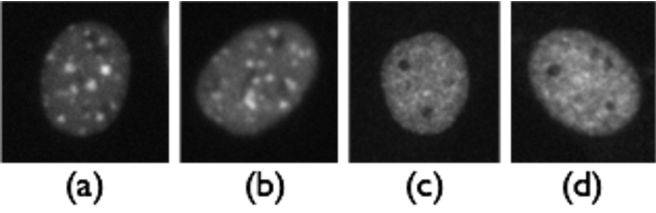
\includegraphics[scale=0.8]{TSA_phenotype.pdf}
\caption{Phenotypic readout on heterochromatin formation: (a)-(b)
  Negative Control, (c)-(d) Signal as observed 
  by an active drug.}
\label{fig:tsa}
\end{figure}

\question[3] Vous êtes consulté comme expert d'analyse d'images par
des biologistes qui veulent analyser une série d'expériences. Ils
utilisent un marqueur qui est informatif pour la compaction de la
chromatine, et ils cherchent à trouver des molécules spécifiques pour
rompre cette organisation. Dans les figures \ref{fig:tsa}.a et
\ref{fig:tsa}.b, nous pouvons observer des images représentatives pour
des cellules normales (sans traitement) et dans les figures
\ref{fig:tsa}.c et \ref{fig:tsa}.d nous pouvons observer l'effet d'une
molécule. Nous ajoutons que la taille et l'intensité moyenne des
cellules n'ont pas de raison d'être différentes entre les deux
conditions. 

Proposer un descripteur spécifique qui nous permettrait de quantifier
cet effet et expliquer votre choix. 
\begin{solution}
Il suffit de détecter des ``spots'' avec des méthodes classiques
(Laplacian of Gaussian, ouvertures morphologiques). Ensuite on peut
calculer les intensités et leurs taille. Alternativement, on peut
utiliser des descripteurs de texture, par exemple la
granulometrie. C'est semblable, mais ça permet de ne pas appliquer un
seuil. 
\end{solution}

\question[3] {\bf Descripteurs de Haralick.}
Les descripteurs de Haralick sont définis à partir de la matrice de
co-occurence normalisée $P_{\Delta_x}$. Nous rappelons que chaque élément
$P_{\Delta_x}(i,j)$ de cette matrice est une estimation de la probabilité jointe
d'observer les valeurs de gris $i$ et $j$ pour des paires de pixels
$(x,x+\Delta_x)$ et $(x,x-\Delta_x)$, avec $\Delta_x \in
\mathbb{Z}^2$. Plus formellement :  
\begin{eqnarray*}
C_{\Delta_x}(i,j) &=& |\{(x,y) \,\,| \,\, y=x \pm \Delta_x, \,\, f(x)=i,
\,\, f(y)=j \}| \\
P_{\Delta_x}(i,j) &=& \frac{C_{\Delta_x}(i,j)}{\sum_i\sum_j C_{\Delta_x}(i,j)}
\end{eqnarray*} 


Le descripteur de ``contraste'' est défini de manière suivante: 
\begin{equation}\label{equ:haralick_contrast}
\vartheta_{\Delta_x} = \sum_i\sum_j(i-j)^2P_{\Delta_x}(i,j)
\end{equation}
Il correspond donc à l'espérance de la différence au carré entre
valeurs de gris pour des pairs de pixels $(x, x \pm \Delta_x)$. 

\begin{parts}
\part Ordonner les images selon $\vartheta_{\Delta_x}  $ dans la
figure \ref{fig:haralick} pour $\Delta_x=(1,0)$. 
\part Ordonner les images dans la figure \ref{fig:haralick} pour la
matrice $P_{\Delta_x}$ moyennée sur $\Delta_x\in \{(1,0), (0,1)\}$ (c'est-à-dire en
direction horizontale et verticale).   
\end{parts}


%\begin{parts}
%\part Expliquer ce que le descripteur $\vartheta_{\Delta_x}$ mesure. 
%\begin{solution}
%L'espérance de la différence entre valeurs de gris au carré pour des
%pixels espacés par $\Delta_x$. 
%\end{solution}
%
%\part Ordonner les images dans la figure \ref{fig:haralick} pour (i)
%$\Delta_x=(1,0)$ et (ii) la matrice moyennée pour $\Delta_x\in
%\{(1,0), (0,1)\}$ (c'est-à-dire en direction horizontale et
%verticale).  
%
%Par exemple, si le descripteur était ``le nombre de pixels noirs'', on
%obtiendrait la solution 1. a - 2. (b,c,d,f) - 3. e. 
%\begin{solution}
%\begin{itemize}
%\item (i) 1.(e,c) - 2.a - 3.f - 4.(b,d)
%\item (ii) 1.e - 2.a - 3.f - 4.(c,d) - 5.b 
%\end{itemize}
%\end{solution}
%
%\end{parts}
%
\begin{figure}[!ht]
\centering
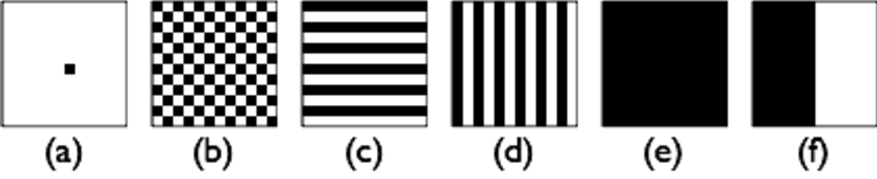
\includegraphics[scale=0.8]{Haralick_question.pdf}
\caption{Images à ordonner selon le descripteur
  \ref{equ:haralick_contrast} }. 
\label{fig:haralick}
\end{figure}

\question[6] {\bf Chaînes de Markov cachées.} 
Beaucoup d'algorithmes liés aux chaînes de Markov cachées sont basés
sur le calcul récursif de certaines probabilités, dont : 
\begin{equation}\label{equ:alpha}
\alpha_t(i) = P(O_1\ldots O_t, q_t=S_i) 
\end{equation}
Ici, $O_t$ est l'observation au temps $t$, $q_t$ est l'état caché au
temps $t$ avec $q_t \in \{S_i\}_{i=1 \ldots N}$ (voire aussi la figure
\ref{fig:hmm}).

\begin{parts}
\part Montrer que $\alpha_1(i)=\pi_i b_i(O_1)$. 
\begin{solution}
\begin{eqnarray*}
\alpha_1 &=& P(O_1,q_1=S_i) \\
&=& P(q_1=S_i)P(O_1 \,|\,q_1=S_i) \\
&=& \pi_ib_i(O_1)
\end{eqnarray*}
\end{solution}
\part Montrer que $\alpha_{t+1}(j) = \left[
  \sum_{i=1}^{N}\alpha_t(i)a_{ij} \right]b_j(O_{t+1})$. 
\begin{solution}
\begin{eqnarray*}
\alpha_{t+1}(j) &=& P(O_1,\ldots, O_t, O_{t+1}, q_{t+1}=S_j) \\
&=& \sum_{i=1}^N P(O_1,\ldots, O_t, O_{t+1}, q_{t+1}=S_j, q_t=S_i) \\
&=& \sum_{i=1}^N P(O_1,\ldots, O_t, q_t=S_i) P(q_{t+1}=S_j \, | \,
q_{t}=S_i) P(O_{t+1} \, | \, q_{t+1}=S_j ) \\
&=& \sum_{i=1}^N \alpha_t(i) a_{ij} b_j(O_{t+1}) \\
&=& \left[\sum_{i=1}^N \alpha_t(i) a_{ij} \right] b_j(O_{t+1}) \\
\end{eqnarray*}
\end{solution}

\part Montrer que $P(O_1, \ldots O_{T}) = \sum_{i=1}^N\alpha_T(i)$. 
\begin{solution}
\begin{eqnarray*}
P(O_1, \ldots O_{T}) &=& \sum_{i=1}^N P(O_1, \ldots O_{T}, q_T=S_i) \\
&=& \sum_{i=1}^N\alpha_T(i)
\end{eqnarray*}
\end{solution}

\end{parts}

Notations : $\pi_i = P(q_1=S_i)$ est la probabilité initiale pour l'état $S_i$,
$a_{ij} = P(q_{t+1}=S_j | q_t=S_i) $ la probabilité de transition,
$b_i(O_t) = P(O_t | q_t=S_i)$ la probabilité d'émission et $T$ la
longueur de la séquence.

Remarque : il convient de rappeler les deux règles fondamentales $P(X)
= \sum_Y P(X,Y)$ et $P(X,Y) = P(X|Y) P(Y)$. 

\begin{figure}[!ht]
\centering
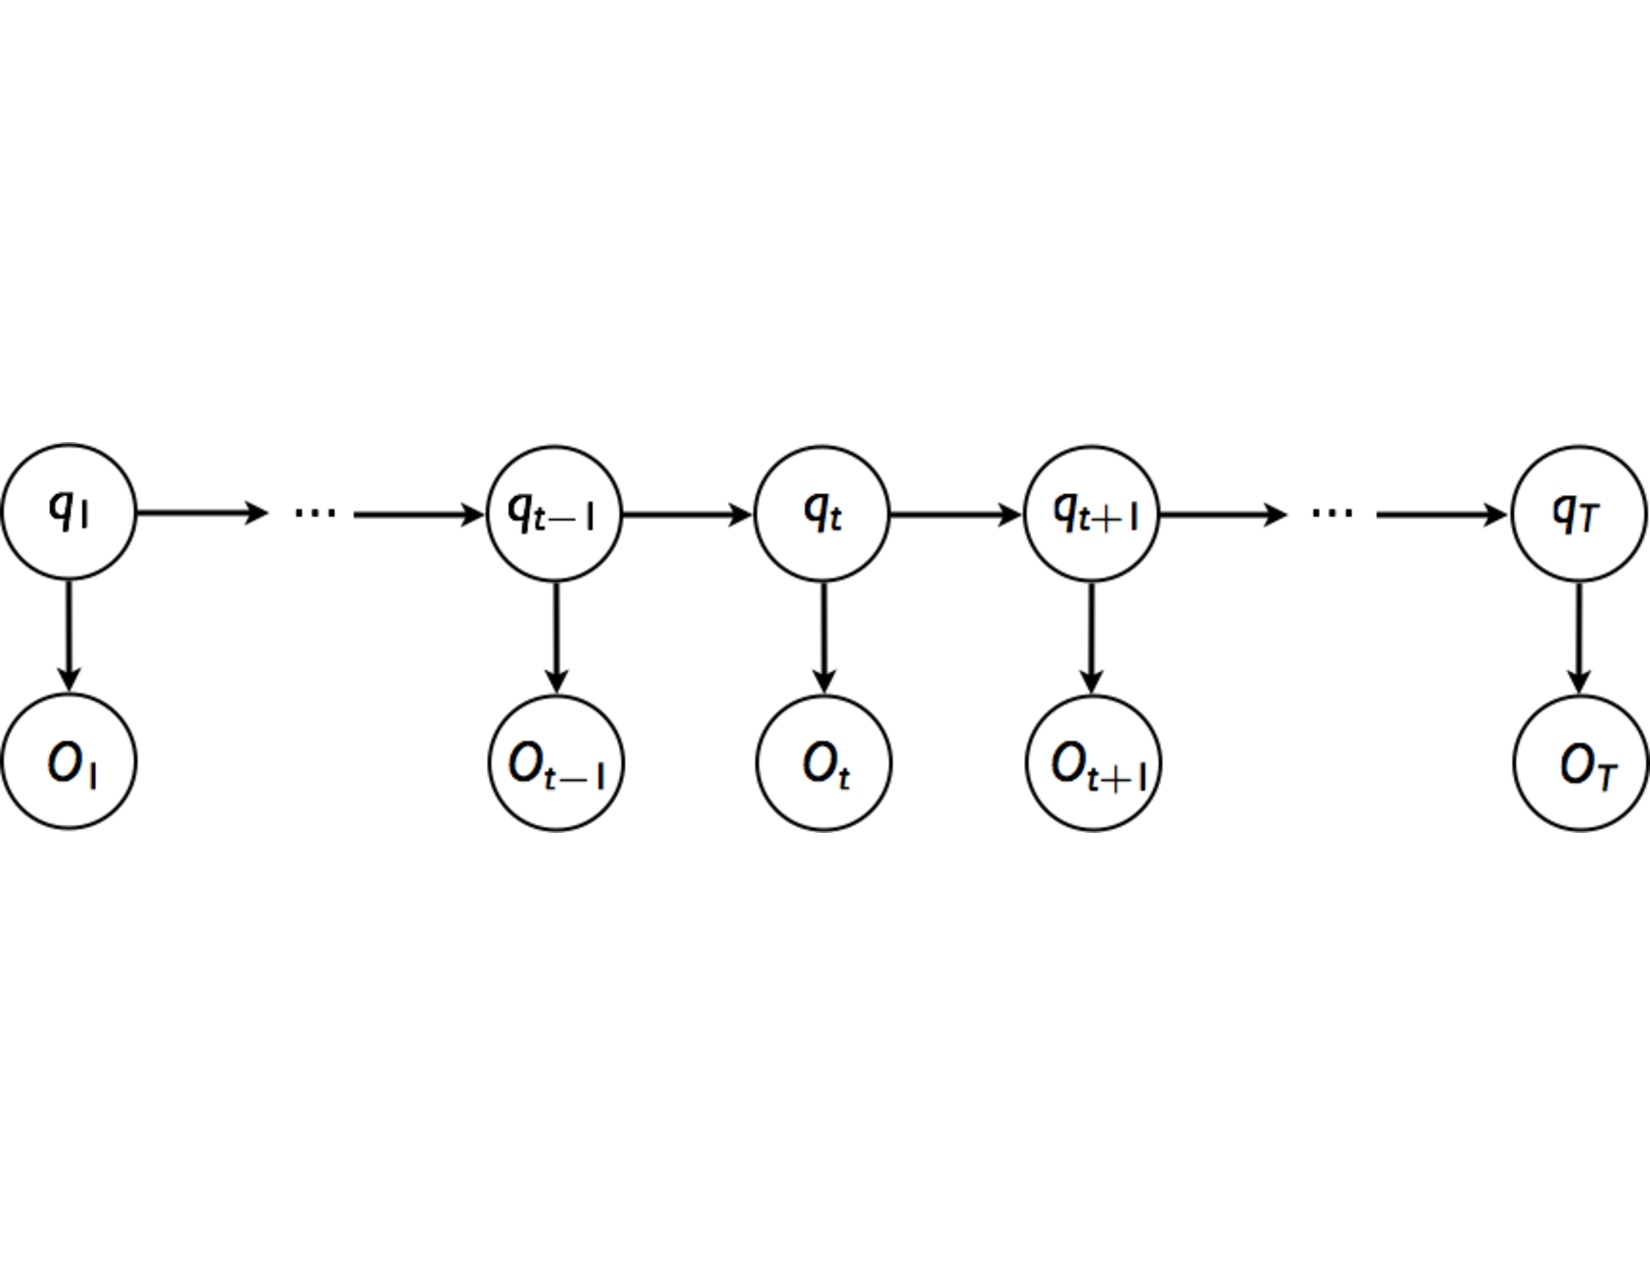
\includegraphics[width=12cm]{HMM_brut.pdf}
\caption{Chaine de Markov cachée.}
\label{fig:hmm}
\end{figure}

%L'estimation des
%paramètres d'une chaine de Markov cachée à partir de séquences
%observées, est basée sur le calcul itératif de certaines probabilités,
%dont : 
%\begin{equation}\label{equ:beta}
%\beta_t(i) = P(O_{t+1}O_{t+2}\ldots O_T |q_t=S_i)
%\end{equation}
%Ici, $O_t$ est l'observation au temps $t$, $q_t$ est l'état caché au
%temps $t$ et $\{S_i\}_{i=1 \ldots K}$ est l'ensemble des états cachés. 


\question[4] {\bf Arbres de décision et forêts aléatoires.}
\begin{parts}
  \part Un arbre de décision définit une partition de l'espace des données en $m$ régions $R_1, R_2, \dots, R_m$. La fonction $f$ qui permet d'associer une étiquette à un objet $x$ peut être écrite sous la forme 
\[ f(x) = \sum_{k=1}^m c_k I_{x \in R_k} \]
où $I_{x \in R_k}$ est une fonction indicatrice qui vaut $1$ si $x \in R_k$ et $0$ sinon. 
Étant donné un jeu d'entraînement $\mathcal{D} = \{x^{i}, y^{i}\}_{i=1, \dots, n}$, comment définit-on $c_k$ 
\begin{itemize}
\item[--] dans le cas d'un problème de classification ?
\item[--] dans le cas d'un problème de régression ? 
\end{itemize}
Remarque : la question porte sur la définition de $c_k$ et non pas sur celle de $R_k$.
\begin{solution}
  \begin{itemize}
  \item classification : classe de la majorité des points du jeu d'entrainement dans cette région.
  \item régression : moyenne des étiquettes des points du jeu d'entrainement dans cette région.
  \end{itemize}
\end{solution}

\part Les forêts aléatoires permettent de combiner plusieurs arbres de décision. Comment transforme-t-on le jeu de données initial pour construire chacun de ces arbres ?
\begin{solution}
  Bootstrap samples + random subset of features (usually square root of the total number of features).
\end{solution}
\end{parts}

\question[5] {\bf Criblage à haut débit.} Le criblage à haut débit ({\it high-througput screening}) permet d'identifier, parmi de nombreuses molécules, lesquelles se lient à une protéine donnée. Le criblage à haut débit virtuel ({\it virtual high-throughput screening}) en est l'équivalent sur ordinateur.
\begin{parts}
  \part Quel est l'intérêt du criblage à haut débit (virtuel ou non) pour la conception de médicaments ?
  \begin{solution}
    Principe clé-serrure : une molécule qui se lie à une protéine cible est un bon candidat à devenir un médicament.
  \end{solution}
  % \part Quel est l'intérêt du criblage virtuel par rapport au criblage non-virtuel ?
  % \begin{solution}
  % Coût du criblage non-virtuel.
  % \end{solution}
  \part Quelles sont les deux grandes familles de techniques que l'on peut utiliser pour faire du criblage virtuel ?
  \begin{solution}
    \begin{itemize}
    \item Machine learning
    \item Docking (simulations)
    \end{itemize}
  \end{solution}
  % \part Quelles sont les limites du concept <<~clé-serrure~>> ({\it key-lock principle}) pour la conception de médicaments ?
  % \begin{solution}
  %   \begin{itemize}
  %   \item Promiscuité des molécules.
  %   \item Ne représentent pas l'intégralité des médicaments (anticorps monoclonaux, thérapie génique, etc.)
  %   \end{itemize}
  % \end{solution}

  \leftskip-2em
  La Figure~\ref{fig:vhts} présente les performances de plusieurs méthodes de criblage virtuel, appliquées à la détection d'inhibiteurs du virus respiratoire syncytial (RSV). Ce virus est la cause la plus fréquente d'infections respiratoires chez les enfants en bas âge (prévalence estimée : 34 millions de cas par an dans le monde chez les enfants de moins de cinq ans). Ici, les molécules sont séparées en deux classes : celles avec une faible activité biologique contre le RSV, et celles avec une forte activité biologique contre le RSV.
  \part Laquelle des méthodes utilisées présente la meilleure performance ?
  \begin{solution}
    Random forests.
  \end{solution}
  \part Dans le cadre du criblage virtuel, est-il préférable d'avoir une forte sensibilité ({\it sensitivity}) ou une forte spécificité ({\it specificity}) ? Sur quelle partie de la courbe ROC doit-on donc se concentrer ?
  \begin{solution}
  On se concentre sur le début de la courbe (faible taux de faux positifs).
  \end{solution}
  % \part Dans le cadre de cette étude, les auteurs ont utilisé les descripteurs dits <<~Mold2~>> pour représenter les molécules. Il s'agit de 777 descripteurs calculés à partir du graphe moléculaire, qui comprennent par example le nombre d'atomes d'oxygène, le poids moléculaire, le nombre de liaisons permetant une rotation, ou la solubilité estimée de la molécule. Quelle autre stratégie pourrait-on utiliser pour représenter les molécules ?
  \part Dans le cadre de cette étude, les auteurs ont utilisé les descripteurs dits <<~Mold2~>> pour représenter les molécules. Il s'agit de 777 descripteurs calculés à partir du graphe moléculaire, qui comprennent par example le nombre d'atomes d'oxygène, le poids moléculaire, le nombre de liaisons permetant une rotation, ou la solubilité estimée de la molécule. Quel risque encourt-on lorsque l'on dispose comme ici de plus de variables (777) que d'échantillons (216) ?
  \begin{solution}
    Extraction systématique de sous-graphes.
  \end{solution}
\end{parts}

% \question[2] {\bf Apprentissage statistique.} 
% \begin{parts}
%   % \part L'algorithme des k plus proches voisins (kNN) prédit pour un échantillon $x$ la classe majoritaire parmi les $k$ plus proches voisins de $x$ dans le jeu d'entraînement. Sur quel(s) paramètre(s) peut-on jouer pour essayer d'améliorer la performance de cet algorithme ?
%   \part Dans le cadre de l'étude présentée à la question précédente (cf. Figure~\ref{fig:vhts}), les auteurs ont séparé leur jeu de données (216 molécules) en un jeu d'entraînement de 163 molécules et un jeu de test de 53 molécules, et rapportent les performances sur le jeu de test. Quelle autre méthode aurait-on pu utiliser pour évaluer les performances des différentes méthodes en maximisant le nombre de molécules utilisées pour l'évaluation ?
%   \part Dans le cadre de cette étude, les auteurs ont utilisé les descripteurs dits <<~Mold2~>> pour représenter les molécules. Il s'agit de 777 descripteurs calculés à partir du graphe moléculaire, qui comprennent par example le nombre d'atomes d'oxygène, le poids moléculaire, le nombre de liaisons permetant une rotation, ou la solubilité estimée de la molécule. Quel risque encourt-on lorsque l'on dispose comme ici de plus de variables (777) que d'échantillons (216) ?
% \end{parts}

\begin{figure}[H]
\centering
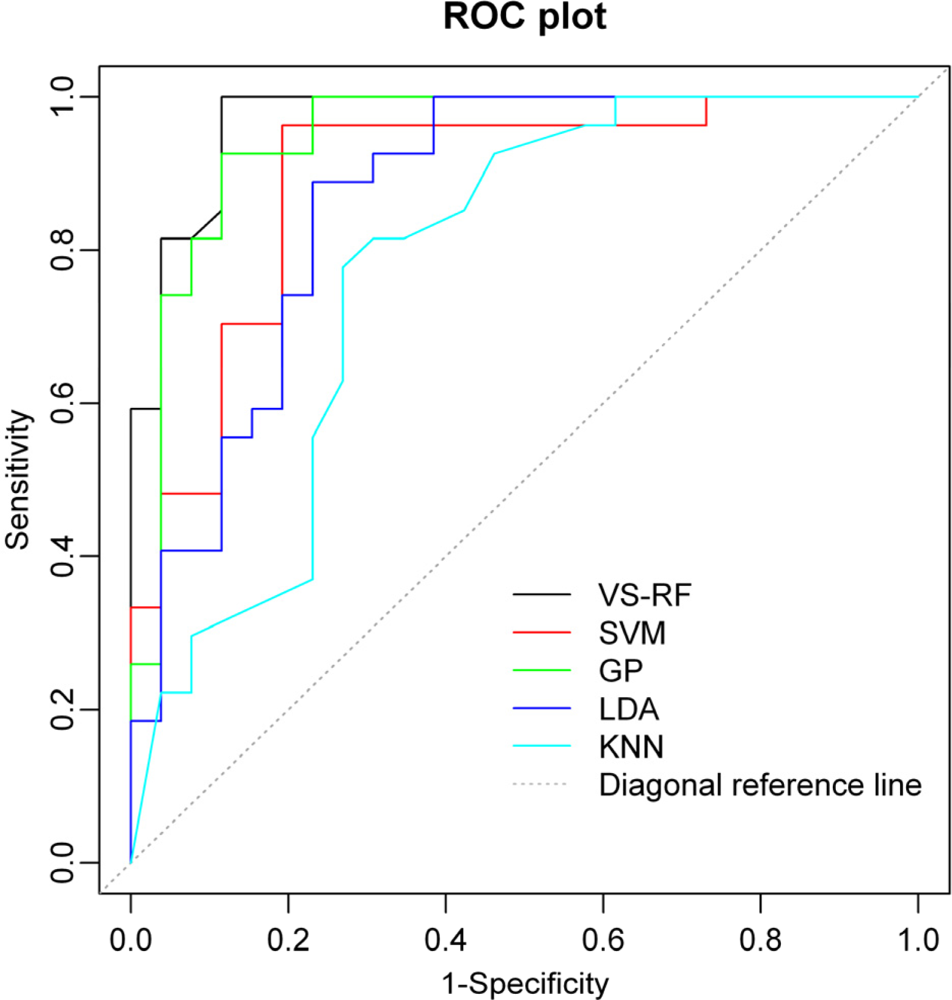
\includegraphics[width=0.5\textwidth]{hao2012_roc}
\caption{Courbes ROC pour plusieurs méthodes de criblage virtuel, sur le jeu de prédiction. \\
Sensitivity = True Positive Rate.
Specificity = 1 - False Positive Rate. \\
VS-RF : Random Forest.
SVM : Support Vector Machine.
GP : Gaussian Process.
LDA : Linear Discriminant Analysis.
kNN : k-Nearest Neighbors.\\
Source: M. Hao, Y. Li, Y. Wang, and S. Zhang, {\it Int. J. Mol. Sci.} 2011, 12(2), 1259-1280.}
\label{fig:vhts}
\end{figure}





\section{Questions sur l'article ``Integrative clustering of multiple genomic data types using a joint latent variable model with application to breast and lung cancer subtype analysis.''}

\question[8] Il existe de nombreux algorithmes qui permettent de faire un clustering d'échantillons sur la base de mesures faites sur ces échantillons (par exemple, le niveau d'expression d'un grand nombre de gènes, ou leur nombre de copies).
\begin{parts}
\part Dans quel but cherche-t-on ici à faire du clustering d'échantillons de tumeurs ?
\begin{solution}
  Découvrir des sous-types de cancer.
\end{solution}
\part Quelle est la limitation de ces techniques que l'article se propose de corriger ?
\begin{solution}
  Impossibilité de faire ce clustering sur des sources de données multiples et hétérogènes.
\end{solution}
\part Quelles sont les deux difficultés rencontrées pour mettre en place cette nouvelle méthodologie ?
\begin{solution}
  \begin{itemize}
  \item Modéliser à la fois la covariance entre sources de données et la structure de variance-covariance au sein de chacune des sources.
  \item Réduire la dimension des données simultanément sur différents jeux de données corrélés.
  \end{itemize}
\end{solution}
\part Comment les différentes classes (clusters) d'échantillons sont-ils modélisés dans cette approche ?
\begin{solution}
  Comme des variables latentes / non-observées.
\end{solution}
\end{parts}

\question[4] Donner la dimension et l'interprétation des termes $\bm{W}$, $\bm{\Psi}$, $\bm{X}$ et $\bm{Z^*}$ dans l'Équation~9.
\begin{solution}
  \begin{itemize}
  \item $\bm{W}: (p_1 + p_2 + \dots + p_m) \times (K-1)$: matrice de projection qui associe l'espace des données à celui des $(K-1)$ directions principales sur lesquelles elles sont projetées.
  \item $\bm{\Psi}: (p_1 + p_2 + \dots + p_m) \times (p_1 + p_2 + \dots + p_m)$: matrice bloc-diagonale composée des matrices de covariance $\Psi_1, \dots, \Psi_m$ interne à chaque type de données.
  \item $\bm{X}: (p_1 + p_2 + \dots + p_m) \times n$: données.
  \item $\bm{Z^*}: (K-1) \times n$: version continue de la matrice $\bm{Z}$ qui assigne chaque échantillon à un cluster.
  \end{itemize}
\end{solution}

\question[6] Figure 2.   
\begin{parts}
\part Comment les auteurs utilisent-ils la Figure 2.B pour déterminer le nombre optimal de clusters ?
\begin{solution}
On évalue à quel point la structure de la matrice est
bloc-diagonale. Le paramètre $K$ qui donne la structure qui ressemble
le plus à une matrice complètement bloc-diagonale est choisi. Ceci
revient à déterminer la ``stabilité''. 
\end{solution}
\part Quelle est la différence entre la Figure 2.A et la Figure 2.D~?
\begin{solution}
Figure 2.A : clustering séparé, Figure 2.D : clustering intégré. 
\end{solution}
\part Que représentent les 3 lignes sur la Figure 2.E ? 
\begin{solution}
Kaplan-Meier: le pourcentage de patients ayant survécu jusqu'au temps
indiqué en abscisse. 
\end{solution}

\end{parts}

\question[8] Figure 3
\begin{parts}
\part % Expliquer la variable utilisée pour le clustering et visualisée
% dans les graphiques de gauche dans la figure 3.A. 
Quelles sont les variables utilisées pour le clustering et visualisées dans les graphiques de gauche de la Figure 3.A ?
\begin{solution}
À gauche le nombre de copies d'ADN (moyennes sur des segments) et à
droite des valeurs d'expression. 
\end{solution}
\part Comparer qualitativement les résultat de clustering présentés dans
les Figure 3.A et 3.B. Qu'impliquent-ils pour la méthode intégrative ?
\begin{solution}
On voit que la structure dans les données est beaucoup mieux capturée
par la méthode intégrative. Notamment le premier cluster. 
\end{solution}
\part Un dendrogramme (tel que montré dans les Figure 3.B et
3.E) permet de visualiser les distances entre clusters au moment de leur fusion. 
Que peut-on dire de la qualité de la méthode utilisée à partir des dendrogrammes montrés
dans les Figure 3.B et 3.E~?
\begin{solution}
Les dendrogrammes montrent la mauvaise qualité de la méthode
hiérarchique utilisée (en dehors du côté intégratif) : chaque sample est assez
différent des autres, mais les clusters de samples sont assez proches
des autres clusters. C'est probablement dû à un mauvais choix de la
méthode d'agglomération. 
\end{solution}
\part Selon les Figure 3.C et 3.F, quelles valeurs de $\lambda$
vous semblent les plus appropriées~? Que contrôle le paramètre $\lambda$~?
\begin{solution}
$\lambda>0$ donne de résultats de meilleure stabilité.  
$\lambda$ pondère le terme de régularisation $L_1$ et contrôle donc la
``sparsity'' de la solution. 
\end{solution}
\end{parts}

\end{questions}

%\begin{enumerate}
%\item 
%\end{enumerate}
\end{document}
